\documentclass[a4paper,12pt,twoside]{article}

%%%%%%%%%%%%
% Packages %
%%%%%%%%%%%%
\usepackage{tabularx}
\usepackage[portuguese]{babel}
\usepackage{packages/sleek}
\usepackage{packages/sleek-title}
\usepackage[acronym]{glossaries}
\usepackage{graphicx}
\usepackage{fancyhdr}

%%%%%%%%%%%%%%
% Glossary %
%%%%%%%%%%%%%%
\makeglossaries
\setglossarystyle{long}
\setglossarystyle{long}
\renewcommand*{\glossaryheader}{%
  \bfseries Termo & \multicolumn{1}{|c}{\bfseries Descrição}\\\hline
}
\renewcommand{\arraystretch}{1.2}
\newglossaryentry{sp}
{
    name=Sistema Pericial (SP),
    description={Sistema de inteligência artificial baseado em regras obtidas através do conhecimento de um perito com o objetivo de resolver problemas específicos de um domínio},
    short=SP,
    text={SP},   
    first={Sistema Pericial (SP)}
}
\newacronym{ia}{IA}{Inteligência Artificial}
\newglossaryentry{IA}
{
    name=IA,
    description={Inteligência Artificial},
    text={\glsentryshort{ia}},      
    first={Inteligência Artificial (\glsentryshort{ia})}
}
\newacronym{vad}{VAD}{Via Aérea Difícil}
\newglossaryentry{VAD}
{
    name=Via Aérea Difícil (VAD),
    description={Situação onde a laringoscopia direta ou máscara facial são difíceis de realizar, podendo levar a complicações graves se não for gerida adequadamente},
    text={\glsentryshort{vad}},      
    first={\glsentrylong{vad} (\glsentryshort{vad})}
}
\newacronym{vadnp}{VADNP}{Via Aérea Difícil Não Previsível}
\newglossaryentry{VADNP}
{
    name=Via Aérea Difícil Não Previsível (VADNP),
    description={Situação onde a laringoscopia direta ou máscara facial são difíceis de realizar, mas que não foram previstas na avaliação pré-anestésica.},
    text={\glsentryshort{vadnp}},      
    first={\glsentrylong{vadnp} (\glsentryshort{vadnp})}
}
\newacronym{ld}{LD}{Laringoscopia Direta}
\newglossaryentry{LD}
{
    name=Laringoscopia Direta (LD),
    description={Procedimento médico que faz uso de um laringoscópio para visualizar detalhadamente a laringe e outras estruturas em volta.},
    text={\glsentryshort{ld}},      
    first={\glsentrylong{ld} (\glsentryshort{ld})}
}
\newglossaryentry{ve}
{
    name=Ventilação espontânea,
    description={Tipo de respiração onde o paciente é capaz de respirar por si só, sem necessidade de auxílio},
    text={ventilação espontânea},      
}
\newglossaryentry{DENDRAL}
{
    name=DENDRAL,
    description={Sistema pericial pioneiro, desenvolvido na década de 1960. Foi utilizado para descobrir a estrutura de compostos químicos com base em espectrómetrias.},
}
\newglossaryentry{MYCIN}
{
    name=MYCIN,
    description={Sistema pericial, desenvolvido na década de 1970 que foi usado para diagnosticar infeções bacterianas. Foi um dos primeiros sistemas a fazer uso de fatores de certeza, entre outros conceitos.},
}
\newglossaryentry{LEMON}
{
    name=LEMON,
    description={Mnemónica usada para avaliar a dificuldade de realizar uma laringoscopia direta.},
    text={LEMON},      
}
\newglossaryentry{MOANS}
{
    name=MOANS,
    description={Mnemónica usada para avaliar a dificuldade de aplicar uma máscara facial.},
    text={MOANS},      
}
\newglossaryentry{RODS}
{
    name=RODS,
    description={Mnemónica usada para avaliar a dificuldade de aplicar um dispositivo supraglótico.},
    text={RODS},      
}
\newglossaryentry{SHORT}
{
    name=SHORT,
    description={Mnemónica usada para avaliar a dificuldade de realizar uma cricotirotomia.},
    text={SHORT},      
}
\newglossaryentry{ds}
{
    name=Dispositivo supraglótico,
    description={Dispositivo médico que é inserido na glote do paciente de forma a manter a sua via aérea aberta, permitindo a ventilação sem a necessidade de intubação traqueal.},
    text={dispositivo supraglótico},      
}
\newglossaryentry{cricotirotomia}
{
    name=Cricotirotomia,
    description={Técnica invasiva de emergência onde é feita uma incisão na membrana cricotireóidea do paciente, permitindo a ventilação.},
    text={cricotirotomia},      
}
\newglossaryentry{SPA}
{
    name=SPA,
    description={Sociedade Portuguesa de Anestesiologia},
    text={SPA},      
}
\newglossaryentry{API}
{
    name=API,
    description={Interface de Programação de Aplicações (do inglês \text{Application Programming Interface}).},
    text={API},      
}
\newglossaryentry{EAMS}
{
    name=EAMS,
    description={\textit{European Airway Management Society.}},
    text={EAMS},      
}
\newglossaryentry{fibroscopia}
{
    name=Fibroscopia,
    description={Procedimento médico que utiliza um tubo fléxivel com uma câmera e luz na extremidade para visualizar as vias aéreas superiores e inferiores.},
    text={fibroscopia},      
}
\glsaddall

%%%%%%%%%%%%%%
% Title-page %
%%%%%%%%%%%%%%
\setlength{\parindent}{15pt}
\logo{./resources/pdf/ISEP.png}
\institute{Insituto Politécnico do Porto}
\faculty{Instituto Superior de Engenharia do Porto}
\department{Departamento de Inteligência Artificial}
\title{Sistema pericial para auxilio na abordagem da Via Aérea em doente submetido a anestesia geral}
\author{
    \textit{Equipa MEIdical}\\
    Danilo \textsc{Silva}  --- nº1250424\\
    João \textsc{Caseiro} --- nº1211334\\
    Luís \textsc{Magalhães} --- nº1100628\\
    Ricardo \textsc{Sousa} --- nº1201856\\
    Tomás \textsc{Pereira} --- nº1210830\\
}


\date{\today}
%%%%%%%%%%%%%%%%
% Bibliography %
%%%%%%%%%%%%%%%%

\addbibresource{./resources/bib/references.bib}

%%%%%%%%%%%%
% Document %
%%%%%%%%%%%%
\begin{document}
    \maketitle
    \pagenumbering{roman}
    \tableofcontents
    \vspace{2em}
    \listoffigures

    \newpage
    \clearpage
    \pagenumbering{arabic}
    \pagestyle{fancy}
    \fancyhf{}

    % --- Headers ---
    \fancyhead[RO]{\textit{SP para auxilio na abordagem da Via Aérea em doente submetido a anestesia geral}}       

    % --- Footers ---
    \fancyfoot[LE]{\textbf{MEIdical}} 

    % --- Page numbers ---
    \fancyfoot[RE,RO]{\thepage}
    
    \section{Introdução}

    O avanço da \gls{IA} tem sido notável em variadissimas áreas. Na medicina, este também é o caso. Na verdade, o uso desta tecnologia na medicina iniciou-se nos anos 60 com o desenvolvimento de um sistema chamado \gls{DENDRAL}~\cite{feigenbaum}, usado para descobrir a estrutura química de um composto através da sua espectrometria. Este é também o primeiro exemplo de um \gls{sp}. 
    
    Os \glspl{sp} são sistemas onde o conhecimento provém de um perito numa determinada área, evitando assim a necessidade de procurar informação em fontes externos, e obtendo-a de uma fonte fiável e aplicada ao problema em questão. O sistema pericial mais conhecido é o \gls{MYCIN}~\cite{shortliffe} que veio revolucionar este tipo de sistemas e definir o padrão para os que se seguiram, introduzindo fatores de certeza e uma arquitetura baseada em regras. Desde então que os \glspl{sp} têm sido aplicados em diversas áreas, desde a medicina, à engenharia, finanças, entre outras.

    Este projeto aborda uma área com muito pouca margem para erro, onde é crucial o perito saber qual o melhor caminho a tomar, podendo uma decisão errada ter consequências muito graves para o paciente. 

    A Anestesiologia é o controlo da dor, da consciência de um paciente, e das suas funções vitais durante um procedimento médico. Quando um paciente está anestesiado, este encontra-se num estado onde tem dificuldade em realizar certas funções autonómicas, como respirar, regular a temperatura corporal, funções gastro-intestinais, entre outros. Devido a isto, um dos principais e mais delicados trabalhos do anestesiologista é o de ventilar o paciente de forma a poder controlar diretamente a respiração do mesmo.


    \subsection{Objetivos}
    Este projeto tem como principal objetivo prever com elevada precisão qual a abordagem da via aérea a aplicar tendo em conta as caracteristicas de cada paciente. Num primeiro momento, baseado nessas mesmas características, será determinado se um doente tem ou não uma \gls{vad}. Nesta fase, o importante é ajudar o perito a evitar uma situação de \gls{vadnp}, avaliando as caracteristicas dos pacientes e atribuindo diferentes pesos a cada uma delas de modo a chegar a uma conclusão mais correta possível.
    
    Numa segunda fase, depois de determinar a abordagem a efetuar, o perito será guiado pelas várias fases do processo de forma a efetuar os passos mais acertados para cada situação específica. Desta forma, o sistema atua como um guia interativode apoio à decisão, garantindo maior segurança e consistência na execução dos procedimentos médicos.

    Para além destes objetivos principais, o projeto visa também:
    \begin{itemize}
        \item Promover a explicabilidade das decisões tomadas através da geração automática de justificações que permitem ao utilizador a qualquer momento obter um esclarecimento do procedimento sugerido ou da conclusão a que foi chegada;
        \item Diminuir o tempo gasto no processo de avaliação inicial ou tomadas de decisão sobre o procedimento adequado, que pode ser crucial para a vida do paciente;
        \item Apoiar a investigação e melhoria contínua, por exemplo, através da recolha e análise de dados anónimos dos pacientes que podem contribuir para estudos futuros e melhoramento do sistema, de forma a ser possível obter resultados cada vez mais precisos.
    \end{itemize}

    Desta forma, este projeto não se limita a uma ferramenta de previsão, mas constitui um sistema completo de apoio à decisão médica.

    \subsection{Fontes de Conhecimento}

    O conhecimento para este projeto foi adquirido na sua grande maioria em reuniões com o perito e documentos fornecidos pelo mesmo. No entanto, foram também analisados trabalhos semelhantes e realizado um estado da arte, além de pesquisas em artigos científicos para melhor ajudar a compreender e contextualizar o problema.

    A principal fonte de conhecimento foi um documento fornecido pelo perito, os Consensos na Gestão Clínica da Via Aérea em Anestesiologia, publicado em 2016 na revista da \gls{SPA}~\cite{consensosva}. Este documento detalha os procedimentos necessários para efetuar as diferentes abordagens da via aérea, utilizando esquemas explicativos e mnemónicas utilizadas pelos peritos para avaliar as características dos pacientes, entre muita outra informação relevante.

    Mesmo assim, o perito foi fundamental para escalrecer dúvidas, explicar muitos dos conceitos presentes no documento e organizar o conhecimnto de forma a que este possa ser utilizada para o desenvolvimento do \gls{sp}.

    \subsection{Perito}

    O perito escolhido para este projeto foi o Dr. Dinis Fernando Pereira Pinheiro Machado da Costa, médico assistente graduado e consultor em anestesiologia do Hospital de Braga. O Dr. Dinis Costa é também formado em Via Aérea pela \gls{EAMS} e integra o grupo de Via Aérea do Hospital de Braga, entre outros. Mestre em Medicina pela Faculdade de Medicina da Universidade de Coimbra, o perito é também formador em Via Aérea e colaborador em várias instituições hospitalares.

    \subsection{Estrutura do Documento}

    Este documento encontra-se organizado em capítulos e sub-capítulos de forma a organizar o seu conteudo da melhor maneira.

    No primeiro capítulo, será feita uma breve introdução ao tema dos \gls{sp}, bem como ao problema em questão, denotando os objetivos traçados para o sistema. Irá também ser feita uma introdução do perito e das fontes de conhecimento utilizadas.

    O segundo capítulo terá como objetivo detalhar todo o conhecimento adquirido e a sua proveniência. Será também apresentado e explicado o fluxograma do conhecimento.\@

    No terceiro capítulo será feita uma breve reflexão sobre o conhecimento adquirido e detalhados quais os próximos passos a tomar no desenvolvimento do projeto.

    \newpage


    \section{Conhecimento Adquirido}
    Nesta secção é apresentado o conhecimento adquirido ao longo do desenvolvimento do sistema, bem como a forma como este foi estruturado e representado no motor de inferência. Será representado e explicado detalhadamente o fluxograma do conhecimento obtido e cada uma das mnemónicas e os seus fatores. De seguida, serão mostrados dois casos de uso e, finalmente detalhadas as sessões com o perito.
    \subsection{Conhecimento}
    \subsubsection{Fluxograma}
    \begin{figure}[H]
        \centering
        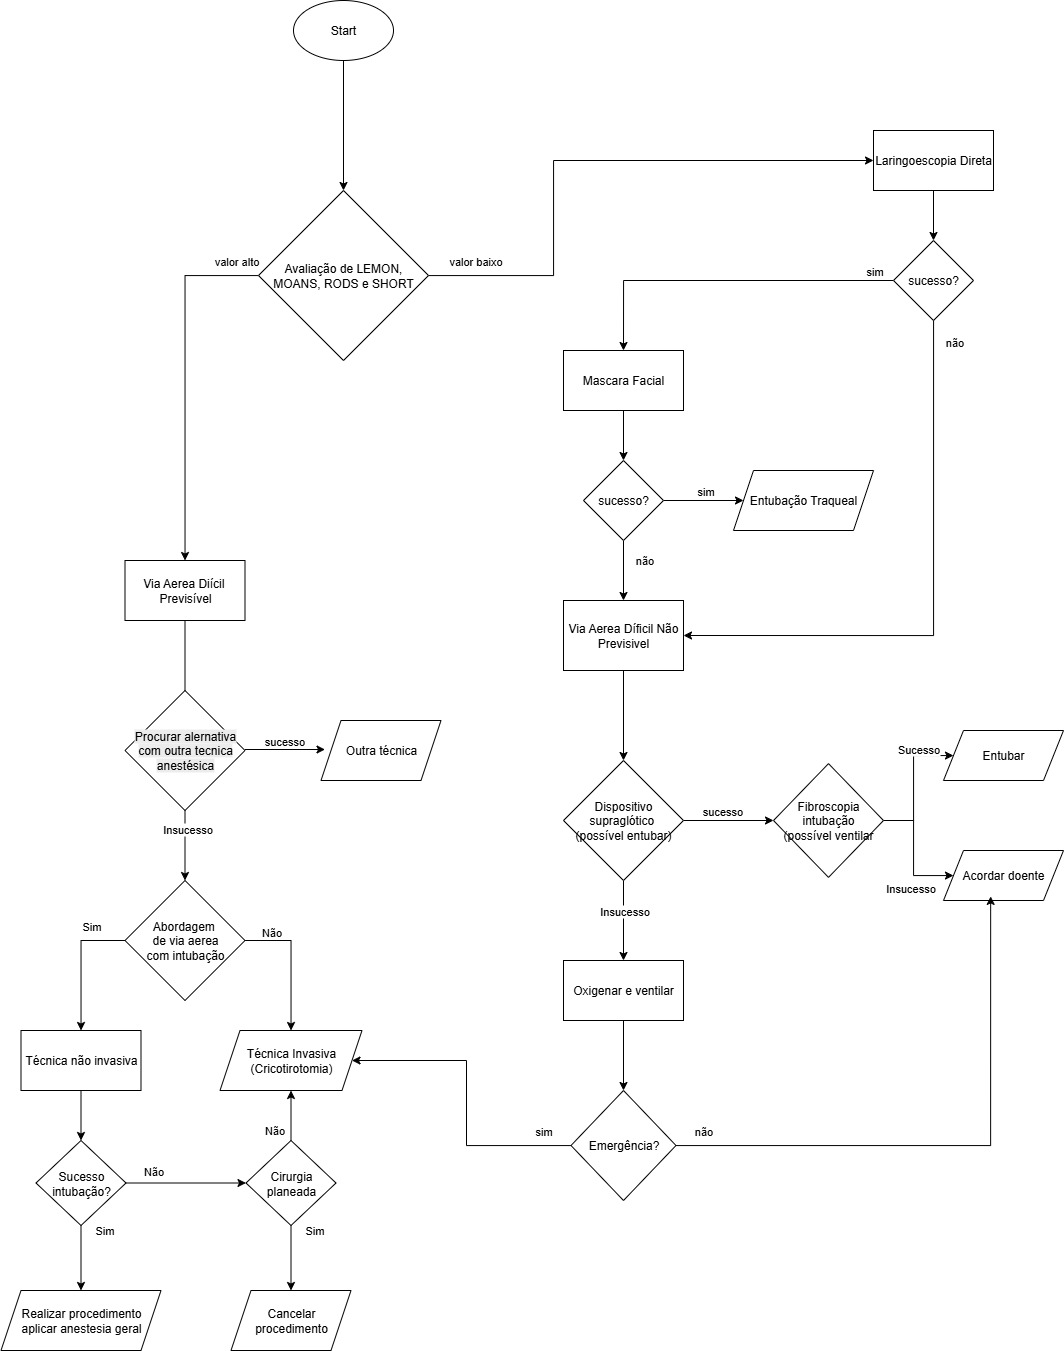
\includegraphics[width=0.8\textwidth]{./resources/pdf/Conhecimento.jpg}
        \caption{Fluxograma do conhecimento.}
        \label{fig:fluxograma}
    \end{figure}

    \subsubsection{Explicação do conhecimento}
    O primeiro passo, e também o mais importante é determinar se o paciente tem uma \gls{vad} ou se a ventilação é possível usando métodos convencionais. Para isso, o perito faz uma série de perguntas com o objetivo de avaliar certas características do paciente. 
    
    \begin{figure}[H]
        \centering
        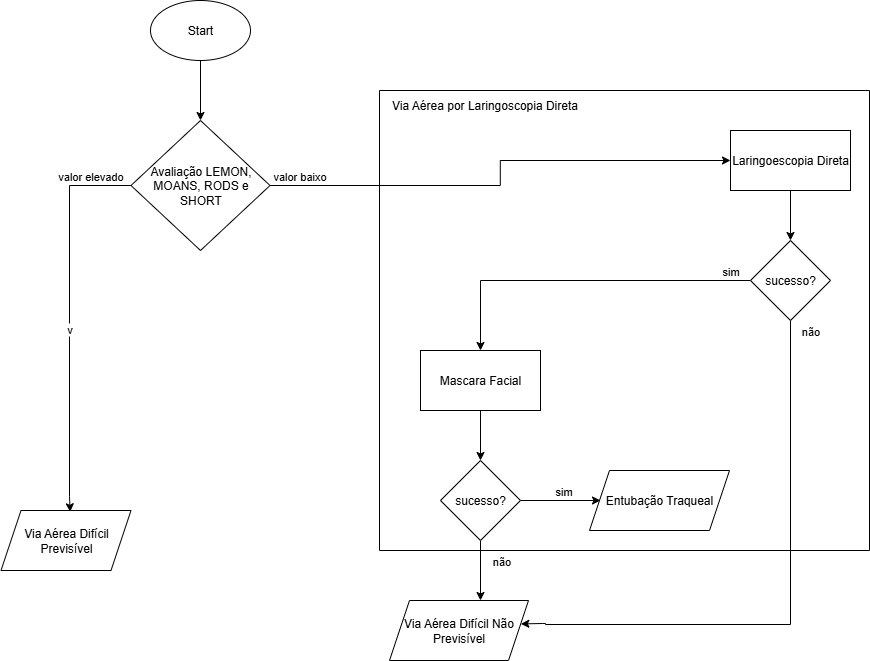
\includegraphics[width=0.8\textwidth]{./resources/pdf/vapld.drawio.png}
        \caption{Fluxograma para determinar abordagem da via aérea.}
        \label{fig:detva}
    \end{figure}

    Normalmente, são utilizadas quatro mnemónicas para avaliar estes critérios: \gls{LEMON}, \gls{MOANS}, \gls{RODS} e \gls{SHORT}~\cite{consensosva}.

    Cada letra de cada mnemónicas equivale a uma característica do paciente que pode dificultar o procedimento. Por exemplo, o letra M da mnemónicas \gls{MOANS} significa \textit{Mask seal}, ou seja, o perito pode ter dificuldade em aplicar a máscara facial pois o paciente pode ter barba densa ou sangue facial que comprometa a operação. Para uma explicação detalhada dos fator de cada mnemónica, ver Secção~\ref{sec:mnemonicas}.

    Sendo assim, cada fator vai ter um determinado peso na decisão final de qual a abordagem da via área do paciente. Por exemplo, o fator ``idade'' da mnemónica \gls{MOANS} (\textit{Age}), refere que o paciente tem mais probabilidade de ter uma \gls{vad} se tiver mais de 55 anos. Isto porque, pacientes com mais idade podem apresentar falta de musculo ou tónus da via aérea o que dificulta a aplicação da máscara facial. No entanto, a idade por si só não é um fator decisivo neste aspeto, pois um paciente pode ter uma idade superior a 55 anos e não apresentar estes problemas. Logo este fator terá um peso menor na decisão final.

    Igualmente, as quatro mnemónicas não têm o mesmo peso na decisão final. A mnemónica \gls{LEMON} é a mais importante, já que avalia a dificuldade de realizar uma \gls{LD}, que é um passo fundamental para a ventilação do paciente.

    Depois do paciente ser avaliado, e de obtermos um resultado proveniente das médias ponderadas das mnemónicas, existem dois caminhos possíveis. Se o valor obtido for baixo, então será considerada uma abordagem de via aérea normal. Será feita uma \gls{LD}, aplicada a máscara facial e, por fim, a intubação traqueal que terminará o processo. Se o valor obtido for elevado, então o paciente tem uma \gls{vad} e serão necessárias utilizar técnicas diferentes, como pode ser visto na Figura~\ref{fig:vad}.

    \begin{figure}[H]
        \centering
        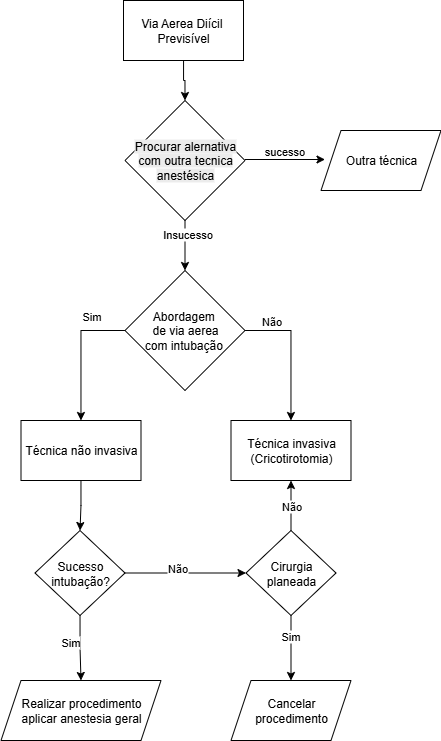
\includegraphics[width=0.5\textwidth]{./resources/pdf/vad.drawio.png}
        \caption{Fluxograma de uma abordagem da via aérea difícil.}
        \label{fig:vad}
    \end{figure}

    Neste caso, o primeiro passo será avaliar se existe outra técnica de ventilação possível. Se for concluido que não, será efetuada uma abordagem da via aérea e intubação com o doente em \gls{ve} e, dependendo do caso, poderá ser necessário utilizar uma técnica invasiva, como a \gls{cricotirotomia}.

    No entanto, devido à subjetividade destas avaliações, é possível que algo corra mal durante o processo de intubação e que este se possa transformar num \gls{vadnp}. Estes são os casos que se pretendem evitar pois podem vir a trazer complicações graves para o paciente, caso não sejam rapidamente resolvidas. O procedimento pode ser visto na Figura~\ref{fig:vadnp}.

    \begin{figure}[H]
        \centering
        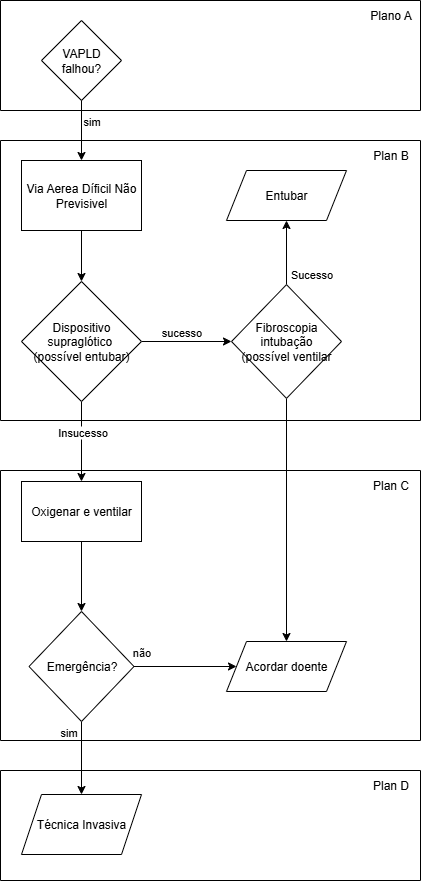
\includegraphics[width=0.4\textwidth]{./resources/pdf/VADNP.drawio.png}
        \caption{Fluxograma de uma via aérea difícil não previsível.}
        \label{fig:vadnp}
    \end{figure}

    Caso este seja o caso, será inserido um \gls{ds}, que permite efetuar a ventilação do paciente sem a necessidade de realizar uma \gls{LD}. Caso tudo corra bem, será então realizada uma \gls{fibroscopia} para verificar se é possível ventilar. Em caso afirmativo, será então realizada a intubação. Caso contrário, o paciente irá ser acordado.

    Por outro lado, se o \gls{ds} concluir que não é possível entubar o paciente, este será acordado e a cirurgia será adiada. No entanto, pode acontecer que o paciente não possa ser acordado e, nestes casos terão de ser efetuados técnicas invasivas como uma \gls{cricotirotomia}. A probabilidade de sucesso desta técnica é determinada pela mnemónica \gls{SHORT}.\@

    \subsection{Explicação das mnemónicas}
    \label{sec:mnemonicas}
    Como já foi brevemente explicado, as mnemónicas são usadas para avaliar vários fatores do paciente que podem contribuir negativamente para a sucesso de uma abordagem normal da via aérea. Cada mnemónica é utilizada para determinar a dificuldade de realizar um determinado procedimento médico associado à intubação do paciente. Dado isto, cada mnemónica tem um peso diferente no resultado final, bem como cada fator dentro de cada mnemónica.
    \subsubsection{LEMON}
    A mnemónica \gls{LEMON} é a mais importante das quatro. Esta avalia a dificuldade de realizar uma \gls{LD}, um paço crucial para a ventilação do paciente.
    \begin{itemize}
        \item L \textrightarrow \textit{ Look Externally}. (Se a via aparenta ser difícil, provavelmente é).
        \item E \textrightarrow \textit{ Evaluate the 3-3-2 rule}. (Distâncias de abertura da boca, mento ao osso hióide e espaço mandibular, em dedos, respetivamente).
        \item M \textrightarrow \textit{ Mallampati Score}. (Grau de exposição de estruturas posteriores da orofaringe).
        \item O \textrightarrow \textit{ Obstruction/Obesity}.
        \item N \textrightarrow \textit{ Neck Mobility}. (A imobilização cervical torna a laringoscopia mais difícil).
    \end{itemize}

    \subsubsection{MOANS}
    A mnemónica \gls{MOANS} avalia a dificuldade de aplicar uma máscara facial.
    \begin{itemize}
        \item M \textrightarrow \textit{ Mask Seal}. (Barba, presença de sangue facial, entre outros, dificultam a selagem da máscara à face).
        \item O \textrightarrow \textit{ Obstruction}. (Alguns fatores como obesidade, gravidez, ou inflamações na via aérea).
        \item A \textrightarrow \textit{ Age}. (Pacientes com idade avançada podem ter uma perda muscular ou de tónus da via aérea elevada).
        \item N \textrightarrow \textit{ No teeth}. (A falta de dentes pode implicar dificuldades na selagem da máscara facial).
        \item S \textrightarrow \textit{ Stiffness}. (Doentes com resistência pulmonar aumentada, como por exemplo, asma).
    \end{itemize}


    \subsubsection{RODS}
    A mnemónica \gls{RODS} avalia a dificuldade de aplicar um \gls{ds}.
    \begin{itemize}
        \item R \textrightarrow \textit{ Restricted Mouth Opening}. (Limitada abertura bocal).
        \item O \textrightarrow \textit{ Obstruction}. (Obstrução abaixo da laringe).
        \item D \textrightarrow \textit{ Disrupted/Distorted Airway}. (Danos na via aérea).
        \item S \textrightarrow \textit{ Stiff Lungs}. (Diminuição da capacidade pulmonar ou da mobilidade cervical).
    \end{itemize}

    \subsubsection{SHORT}
    A mnemónica \gls{SHORT} avalia a dificuldade de realizar uma \gls{cricotirotomia}.
    \begin{itemize}
        \item S \textrightarrow \textit{ Surgery}. (Cirurgia prévia na via aérea).
        \item H \textrightarrow \textit{ Hematoma}.
        \item O \textrightarrow \textit{ Obstruction}.
        \item R \textrightarrow \textit{ Radiation}. (Radiação prévia).
        \item T \textrightarrow \textit{ Trauma}.
    \end{itemize} 

    \subsection{Casos de Uso}
    Para melhor entender o domínio, irão ser apresentados dois casos de uso, um onde o paciente tem uma \gls{vad} e outra onde é necessária uma abordagem de \gls{vadnp}.
    \subsubsection{Caso de Uso 1 --- Via Aérea Difícil}

    \begin{figure}[H]
        \centering
        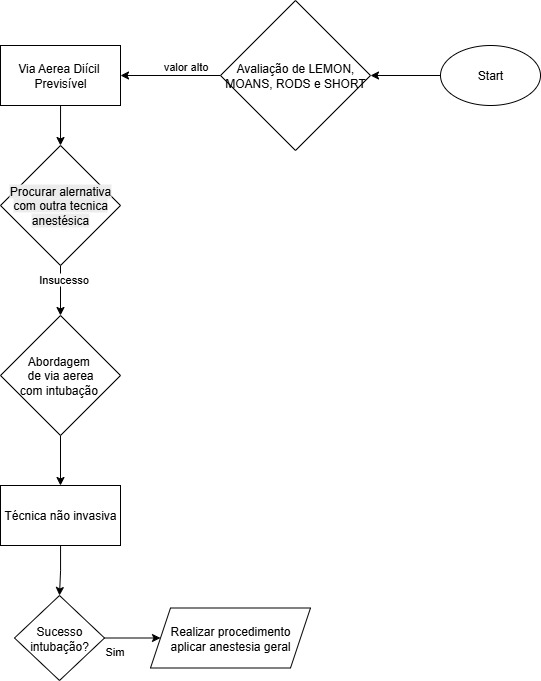
\includegraphics[width=0.5\textwidth]{./resources/pdf/casoDeUso1.jpg}
        \caption{Caso de uso 1 --- Via Aérea Difícil.}
        \label{fig:caso1}
    \end{figure}

    Consideremos o caso hipotetico de um paciente com as seguintes caracteristicas:
    \begin{itemize}
        \setlength{\itemsep}{2pt} 
        \setlength{\parskip}{0pt} 
        \setlength{\parsep}{0pt} 
        \item Idade: 60 anos
        \item Sem dentes
        \item Distância mento-hióide: 1 dedo
        \item Mobilidade cervical: normal
        \item Com barba densa
        \item Sem obstrução da via aérea
        \item Com antecedentes de cirurgia prévia na via aérea
    \end{itemize}

    Com base nestas caracteristicas, o sistema irá então avaliar a dificuldade de realizar uma abordagem normal da via aérea. O paciente tem uma idade acima do limite, no entanto este fator tem um peso baixo na decisão final. Contudo, o facto de este não possuir dentes e ter uma barba densa são fatores muito conisderáveis na aplicação da máscara facial, bem como uma distância mento-hióide muito curta. O sistema irá então concluir que é necessária uma abordagem de \gls{vad}.
    
    De seguida, o perito irá avaliar se existe outra técnica de ventilação possível no momento. Neste caso hipotético, o perito conclui que não existe, por isso será realizada uma abordagem de via aérea com intubação com recurso a uma técnica não invasiva, como uma \gls{fibroscopia}. O procedimento realiza-se com sucesso e é então possível aplicar anestesia geral. O fluxograma para este caso pode ser visto na Figura~\ref{fig:caso1}.

    Em relação às regras ativadas por este caso de uso, em primeiro lugar serão acionadas as regras de criação dos fatores. Neste caso, os fatores correspondentes à idade (LEMON-A), ausência de dentes (MOANS-N), barba densa (MOANS-M), distância mento-hióide reduzida (LEMON-E) e antecedentes de cirurgia na via aérea (SHORT-S). De seguida, será efetuado o cálculo de previsão de via aérea utilizando valores de certeza. Neste exemplo, o valor obtido será acima do estipulado como valor máximo para via aérea normal para a mnemónica MOANS e, dado isso, irá ativar a regra correspondente, chegando então a uma conclusão intermédia. A partir daqui, o sistema irá interativamente, para cada processo, perguntar ao utilizador pelo sucesso/insucesso do mesmo e com base na sua resposta ativar as regras correspondentes até chegar a uma conclusão final. Por exemplo, após o insucesso de ``Realizar uma abordagem da via aérea com intubação``, o sistema irá acionar uma regra para iniciar o processo de ``Técnica não invasiva``, e retornar ao utilizador a abordagem recomendada. Após o processo, o utilizazador seleciona o sucesso da opção no sistema e, será acionada a regra final, que cria a conclusão ``Aplicar anestesia geral``.

    \subsubsection{Caso de Uso 2 --- Via Aérea Difícil Não Previsível}

    \begin{figure}[H]
        \centering
        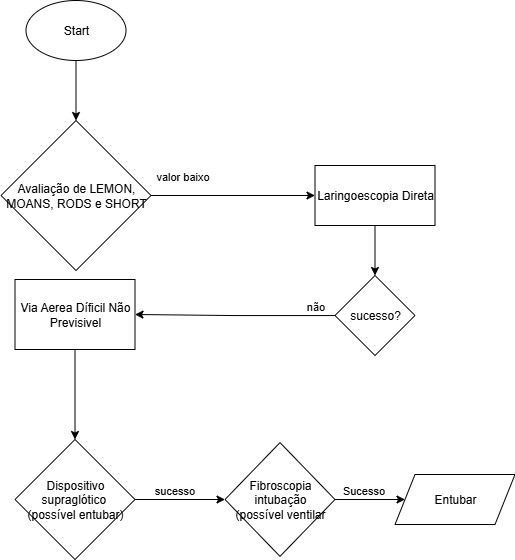
\includegraphics[width=0.4\textwidth]{./resources/pdf/casoDeUso2.jpg}
        \caption{Caso de uso 2 --- Via Aérea Difícil Não Previsível.}
        \label{fig:caso2}
    \end{figure}

    Consideremos agora o seguinte caso hipotético de um paciente com as seguintes caracteristicas:
    \begin{itemize}
        \setlength{\itemsep}{2pt} 
        \setlength{\parskip}{0pt} 
        \setlength{\parsep}{0pt} 
        \item Idade: 30 anos
        \item Sem barba
        \item Com dentes
        \item Distância mento-hióide: 3 dedos
        \item Mobilidade cervical: normal
        \item Sem obstrução da via aérea
        \item Sem antecedentes de cirurgia prévia na via aérea
    \end{itemize}

    Neste caso, não existe qualquer indicio relevante que indique que o paciente possa ter uma \gls{vad}. O paciente é jovem, não apresenta barba, tem dentes, uma distância mento-hióide normal e não apresenta qualquer obstrução da via aérea. Dado isto, o sistema irá então concluir que é possível realizar uma abordagem normal da via aérea. 
    
    No entanto, durante o procedimento de \gls{LD}, algo corre inesperadamente mal e o procedimento transforma-se numa \gls{vadnp}. O perito tenta, com um \gls{ds} verificar se a intubação é possível e com uma \gls{fibroscopia} se o paciente pode ser ventilado. Ambos os procedimentos têm sucesso e então o sistema conclui que o paciente pode ser intubado. O fluxograma para este caso pode ser visto na Figura~\ref{fig:caso2}.

    Para este exemplo, o processo é muito similar. Neste caso, não são ativadas nenhumas regras para criação dos fatores e, por isso, é acionada a regra para iniciar o processo de \gls{LD}. O processo será semelhante ao descrito no caso anterior, recomendando ao utilizador o processo seguinte, o utilizador indicando o sucesso/insucesso das operações e, consoante essa avaliação, será disparada a regra correspondente que irá iniciar o processo seguinte até o sistema chegar a uma conclusão final.

    \subsection{Sessões de Aquisição do Conhecimento}
    \subsubsection{Primeira sessão}
    \begin{tabularx}{0.6\textwidth}{@{}lX@{}}
        \textbf{Data:} & 23/09/2025 \\
    \end{tabularx}

    A primeira sessão foi uma sessão de apresentação do perito à equipa e vice-versa. Foram colocadas em cima da mesa vários problemas dentro da área de anestesia que seriam interessantes de abordar com um \gls{sp}, no entanto, dado á proximidade profissional do perito com a área da anestesia por via aérea, foi decidido que seria este o tema a abordar. Foi feita à equipa uma apresentação e explicação dos conceitos básicos do domínio, e foi fornecido um documento (\cite{consensosva}) que o perito considerou de extrema relevância para o desenvolvimento do conhecimento do projeto. A equipa ficou com a tarefa de analisar o documento e preparar questões para a próxima sessão.

    \subsubsection{Segunda sessão}
    \begin{tabularx}{0.5\textwidth}{@{}lX@{}}
        \textbf{Data:} & 28/09/2025 \\
    \end{tabularx}

    O principal objetivo da segunda sessão era esclarecer dúvidas sobre o documento fornecido anteriormente. Com a ajuda do perito, foi possível sistematizar e compreender os vários esquemas e fluxogramas e quais os pontos mais relevantes a serem tidos em conta. Foram também discutidas as mnemónicas e a sua importância na avaliação do paciente.

    \subsubsection{Terceira sessão}
    \begin{tabularx}{0.5\textwidth}{@{}lX@{}}
        \textbf{Data:} & 4/10/2025 \\
    \end{tabularx}

    Para a terceira sessão, a equipa preparou um primeiro fluxograma do conhecimento, baseado no que tinha sido discutido anteriormente. Após revisão do mesmo com o perito, foram feitas várias alterações ao mesmo. Foi também discutida a possibilidade de atribuir pesos a cada fator das mnemónicas, bem como a cada mnemónica em si de forma a que o sistema possa ser o mais preciso na sua avaliação.

    \subsubsection{Quarta sessão}
    \begin{tabularx}{0.5\textwidth}{@{}lX@{}}
        \textbf{Data:} & 11/10/2025 \\
    \end{tabularx}

    Sessão final para validação do conhecimento adquirido. Também foram esclarecidas algumas dúvidas finais e ajustados alguns valores probabilísticos referentes aos pesos das mnemónicas e dos seus fatores.

    \newpage


    \section{Reflexões finais}
    \subsection{Adequação do trabalho ao meio envolvente}
    O sistema desenvolvido apresenta uma clara adequação ao contexto hospitalar, uma vez que foi concebido para apoiar rapidamente e com clareza profissionais de saúde na avaliação e gestão de vias aéreas difíceis, um processo crítico em ambientes de urgência e anestesia. A forma como o projeto foi desenvolvido facilita a sua integração em infraestruturas existentes, sem necessidade de grandes alterações nos sistemas em uso, apenas sendo necessário o acesso do utilizador a um website onde rapidamente este pode iniciar o processo de auxilio de decisão. Além disso, as justificações do motor de inferência contribuem para a transparência das decisões clínicas, reforçando a confiança dos profissionais e promovendo a segurança do doente. Assim, este sistema demonstra um elevado potencial de aplicação prática em hospitais e outras instituições de saúde, tanto no apoio à decisão em situações críticas, como até mesmo na formação médica.
    \subsection{Próximos objetivos}
    O principal passo seguinte a tomar será ajustar os valores probabilísticos dos pesos das mnemónicas e dos seus fatores para valores definitivos.
    Com o conhecimento adquirido, o próximo passo será a implementação do \gls{sp} em si. Já foi feita a implementação das \glspl{API} tanto em Prolog como em Java, usando Spring Boot neste último caso. De seguida, será desenvolvida o \textit{frontend} do sistema e serão codificadas as várias regras do conhecimento tanto em Prolog como em Drools.
    \subsection{Conclusão}
    O conhecimento adquirido tem um grande impacto na precisão do \gls{sp}, ainda mais numa área tão sensível. A ajuda do perito foi fundamental durante todo o processo, desde a aquisição, até à validação do mesmo.

    \newpage

    \printglossary

    \newpage

    \nocite{*}
    \printbibliography
\end{document}
